\chapter{MOEA-RS}
O método proposto nesse trabalho consiste de um sistema de recomendação multiobjetivo com baseado em conteúdo para filmes. O sistema apresenta os mesmos componentes que um sistema de recomendação baseado em conteúdo tradicional, a principal diferença está na etapa de filtragem, onde, ao contrário dos sistemas tradicionais que utilizam abordagens comuns de filtragem, o sistema proposto no trabalho utiliza um MOEA para buscar os itens que otimizem os critérios definidos. O diagrama de fluxo pode ser visto na Figura~\ref{fig:fluxo} . Cada componente do sistema será descrito na seção abaixo. Por fim, será descrita as atividade definidas para execução deste trabalho.
\begin{figure}[h!]
   
    \centering
    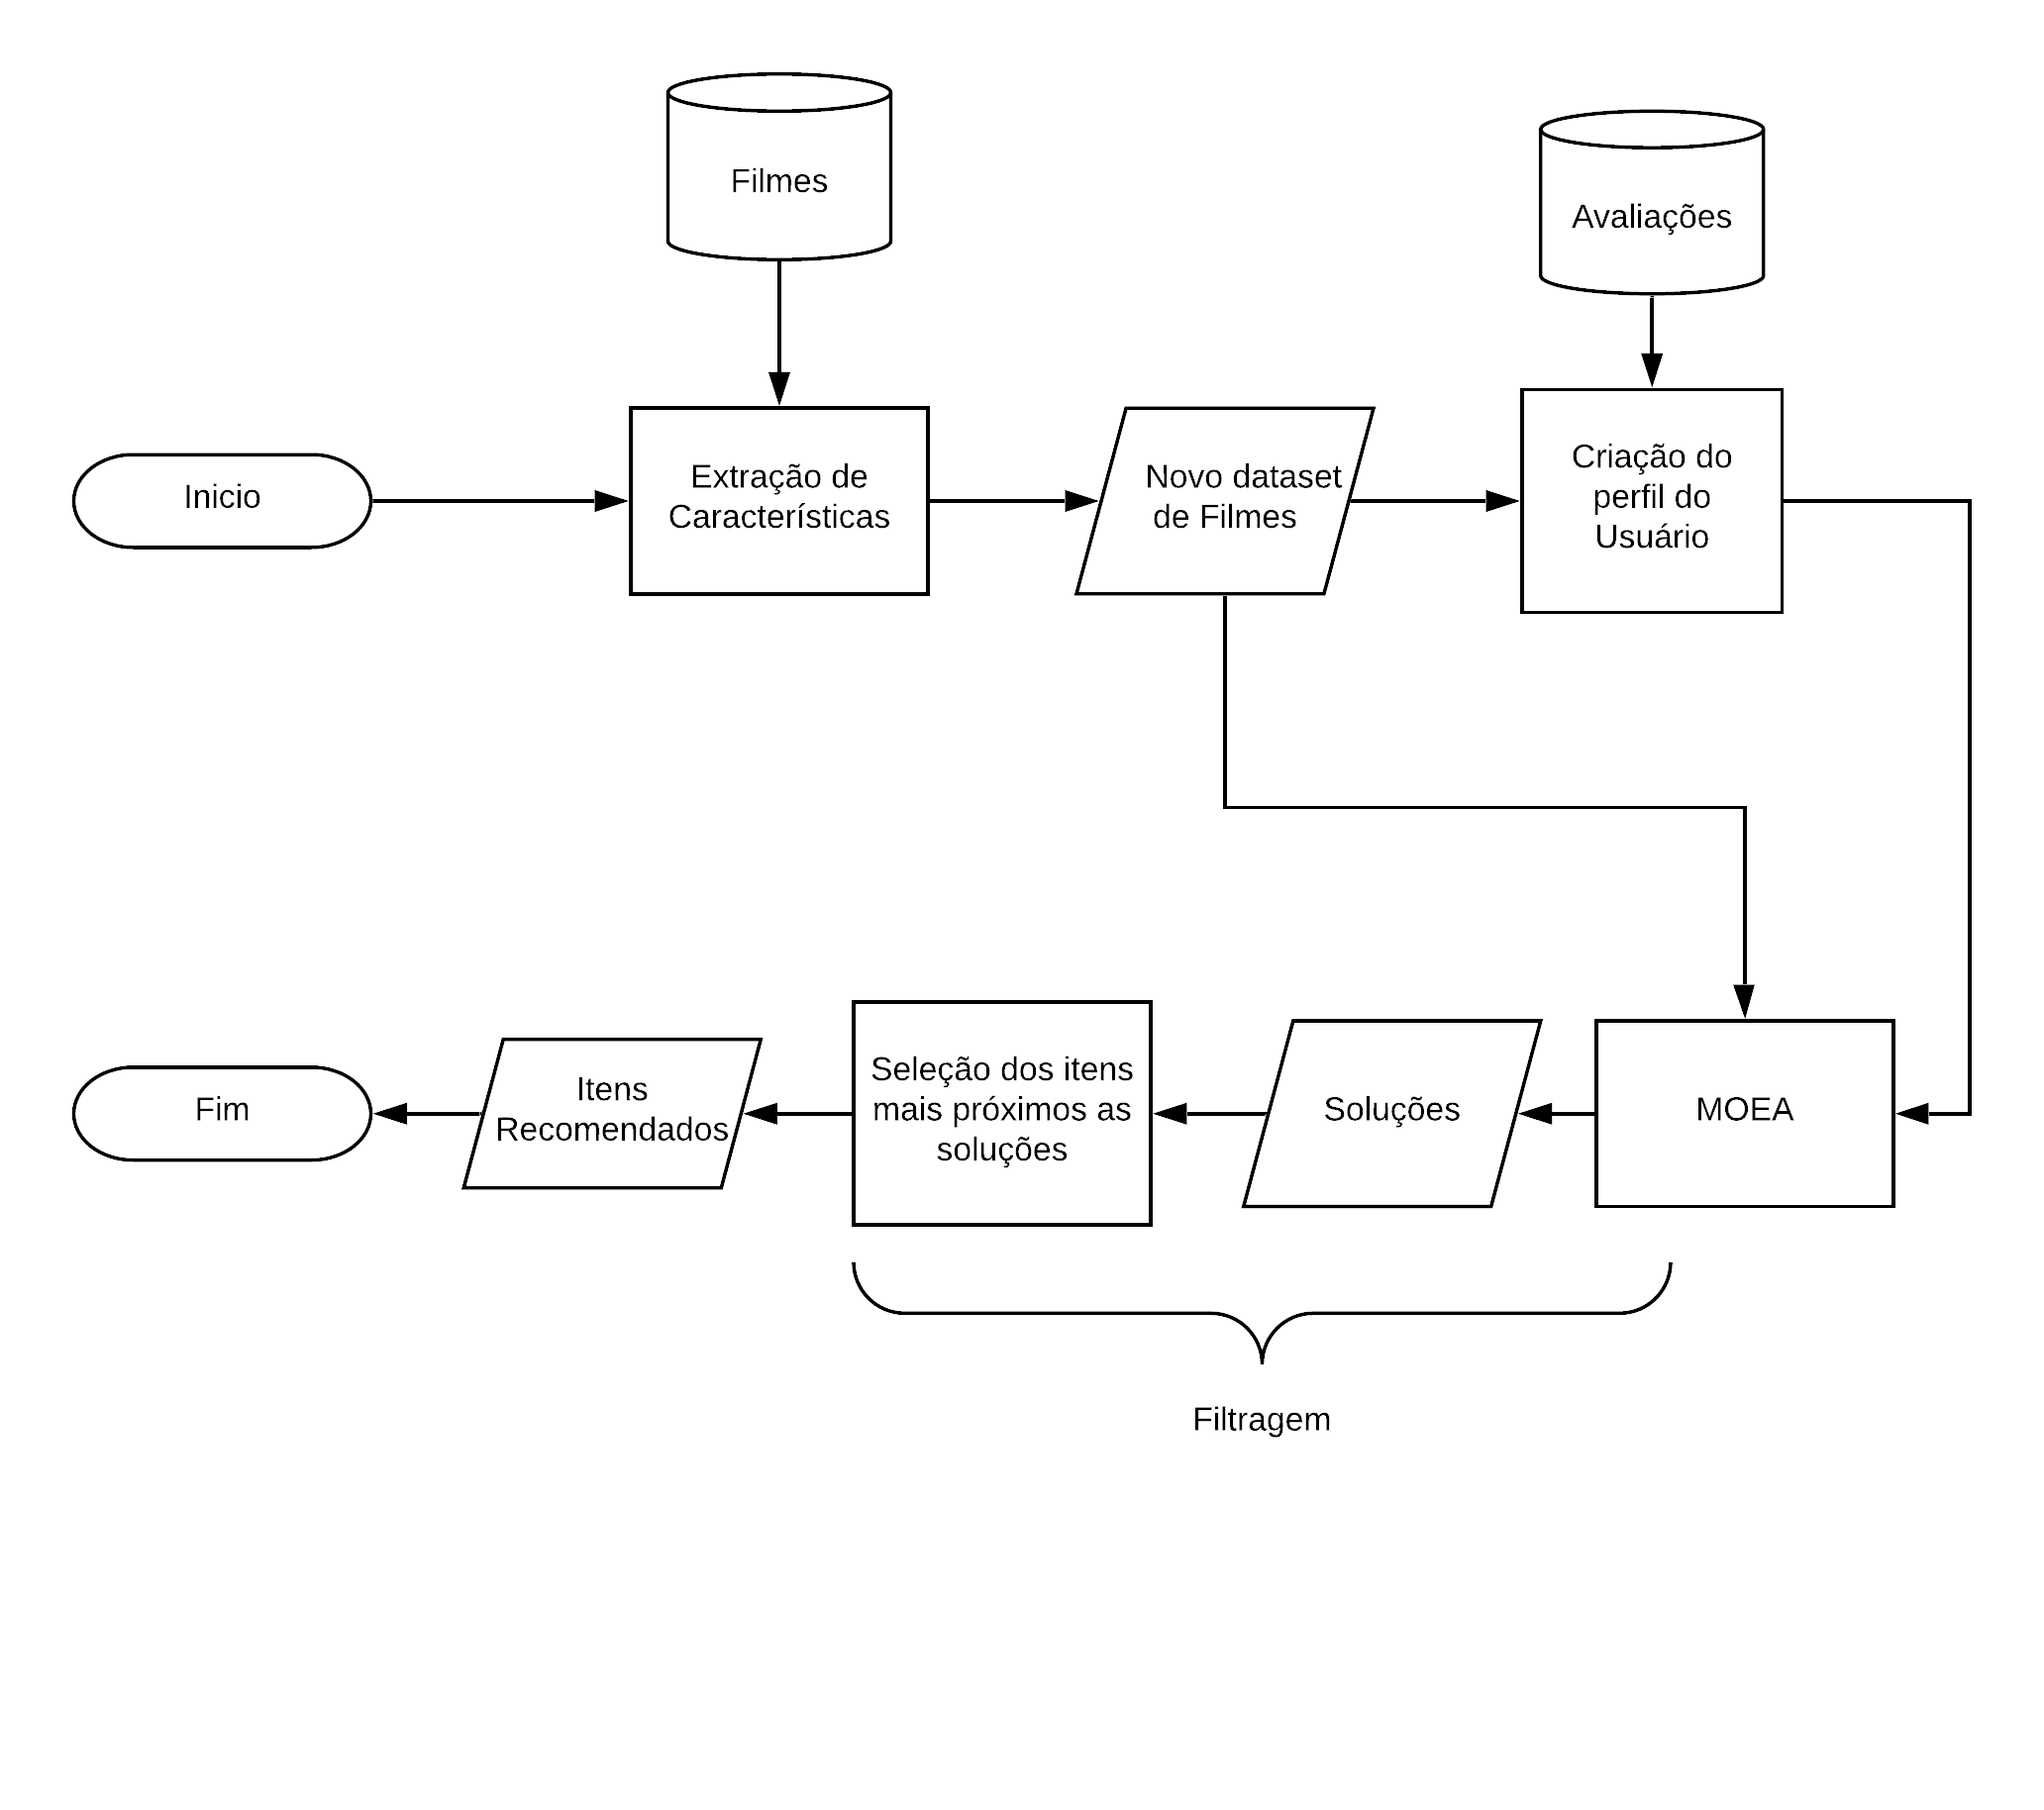
\includegraphics[width=14cm]{Imagens/algoritmo_fluxo.png}
   \caption{Diagrama de fluxo do MOEA-RS}
    \label{fig:fluxo}
    
\end{figure}

\section{\textit{Datasets} de Filmes}
Esse método utilizará dois \textit{datasets} para auxiliar o sistema de recomendação. O primeiro \textit{dataset} é o MovieLens\cite{harper2016movielens}, que contém a avaliação de diversos usuários sobre filmes, essas avaliações foram obtidas a partir da iteração desses usuários com a plataforma online do Movielens. O segundo \textit{dataset} é o IMDB, que contém informações sobre diversos filmes, como sinopse, atores, diretores e etc~\cite{imdb}. 

Como o sistema de recomendação proposto é um sistema baseado em conteúdo, o \textit{dataset} com as avaliações será divididos em diversos \textit{datasets}, onde cada \textit{dataset} resultante terá as avaliações de apenas um usuário.

\section{Análise de conteúdo}
Esse componente é responsável por transformar a representação de um filme em um vetor de características. No IMDB, os filmes são representados por diversos tipos de atributos, porém, os atributos que serão utilizados (\textit{e.g.}, sinopse, gêneros, titulo, diretores, etc ), são textuais e categóricos, portanto, o analisador de conteúdo terá que ser capaz de transformar informação textuais e categóricas em um vetor de valores numéricos. 

Nesse trabalho, foi proposta a seguinte estrategia para extração de características de atributos textuais : primeiramente, serão identificadas as palavras chaves daquele atributo, para isso, será utilizado o algoritmo Rake~\cite{inbook}, que busca encontrar palavras chaves com base na ocorrência daquela palavra nos textos e na sua co-ocorrência com outras palavras. Após a extração das palavras chaves, para cada filme, será atribuido um peso relacionado a uma palavra, esse peso será calculado utilizando o método TF-ID~\cite{salton1989automatic}, que busca calcular a relevância de uma palavra em um texto com base na sua ocorrência em outros textos. Assim, para cada atributo textual, será gerado diversos atributos numéricos, onde cada atributo representa a relevância de uma palavra chave para aquele filme.

Com relação aos atributos categóricos, será utilizada a seguinte estrategia: para cada atributo categórico, cada valor possível será transformado em um atributo numérico, onde seu valor é igual a 1 caso o filme possua aquela categoria e 0, caso contrário.

Portanto, o resultado do analisador de conteúdo corresponde a um novo \textit{dataset}, onde cada linha representa um item e todos os atributos do item serão valores numéricos. Esse \textit{dataset} será utilizado componente de construção do perfil dos usuários e na filtragem.


\section{Construção do perfil usuário}
Esse componente recebe como entrada um conjunto de \textit{datasets}, onde cada \textit{dataset} corresponde às avaliações de um usuário sobre diversos filmes, além do \textit{dataset} resultante análise de conteúdo. Como resultado, o componente irá construir um modelo de regressão \(R_u(i)\) para cada usuário \(u\), que representará a chance de um usuário gostar de um filme \(i\). Esses modelos serão utilizados no componente de filtragem.

O modelo de regressão utilizado neste trabalho foi o modelo \textit{Ridge}, que é um modelo de regressão linear que utiliza a função de erro de mínimos quadrados com a norma \(l^2 \) como regularização \cite{scikit-learn}. Neste modelo, o objetivo é minimizar a equação \ref{lw}, onde w é o vetor peso, X é o vetor de características, Y é o valor alvo e $\alpha$ é um valor positivo indicando a força de regularização.
\begin{equation}
\label{lw}
    l(w) = ||y - Xw||^2_2 + \alpha * ||w||^2_2
\end{equation}

\section{Filtragem}
Para executar a filtragem, o componente responsável pela recomendação dos itens, a recomendação será modelada como um problema multiobjetivo, sendo que, os itens recomendados serão aquele que otimizem os critérios definidos. 

\subsection{Problema de Recomendação}
O sistema de recomendação proposto neste trabalho busca recomendar itens com três objetivos: estimativa da avaliação do usuário sobre o item, avaliação geral do item, novidade e diversidade.

A estimativa da avaliação do usuário é obtida a partir do modelo gerado no componente de aprendizado de perfil, assim, o objetivo é dada pela função:

\begin{equation}
\label{F1}
    F1(i) = R^*(u, i),
\end{equation}

onde \(R*\) é a estimativa de avaliação do usuário u sobre o item i. A novidade de um item  é dado pela seguinte equação \cite{zhang2013}:
\begin{equation}
\label{F2}
    F2(i) = \min_{j \in A_u} (1 - similaridade(i,j)),
\end{equation}        

sendo \(A_u\) o conjunto de itens que foram avaliados pelo usuário u, portanto, essa função objetivo pode ser interpretada como a similaridade entre o item recomendado e os itens que já foram avaliados pelo usuário. A terceira função - a diversidade - corresponde a uma função que busca relacionar um item recomendado ao outros itens da lista de recomendação, essa função calcula o quão diferente é o item em comparação aos itens da lista. O propósito desse é garantir que a lista de recomendação seja mais heterogênea. A diversidade de um item em comparação aos outros itens da lista pode ser calculada da seguinte forma:
\begin{equation}
\label{F3}
    F3(i) = \frac{1}{|P-i|}\sum_{j \in P - i} (1 - similaridade(i,j)), 
\end{equation}

onde P é o conjunto de itens a serem recomendados, que nesse método será a população gerada pelo MOEA. 

Portanto a recomendação pode ser modelado como um problema de otimização multiobjetivo(minimização), onde deve se encontrar um item \(i\) para um usuário \(u\), que otimize as seguintes equações:

\label{problema}
\[
\left\{
        \begin{array}{ll}
          \min - F1(i) = R^*(u, i) \\ 
          \min  - F2(i) = \min_{j \in A_u} (1 - similaridade(i,j)) \\ 
          \min - F3(i) = \frac{1}{|P| - 1}\sum_{j \in P - i} (1 - similaridade(i,j))
        \end{array}
      \right.
\]
Para isso, a solução do problema foi definida como um vetor que representará o item, onde cada elemento desse vetor corresponde a uma característica do item.

\subsection{Processo de Recomendação}

A recomendação é feita a partir da execução de um MOEA para solucionar o problema descrito na seção anterior. Vale ressaltar que o MOEA não vai executar uma busca dentro do conjunto de itens, a busca será feita em um conjunto \(S\) onde, sendo \(s = [s_1, s_2, ..., s_m ]\), se \(s \in S\), então  \(l_i< s_i < u_i\), onde \(l_i\) e \(u_i\) é o menor e o maior valor da característica \(i\) do item, respectivamente, e  \(m\) é o número de características do item.  Em outras palavras, a espaço de busca do MOEA contém o espaço de itens, mas, diferentemente do espaço de itens, esse espaço de busca é continuo.

O motivo para que a busca não seja feita no espaço de itens é que cada solução, gerada durante a execução do MOEA, teria que ser comparada aos itens do \textit{dataset}, o que aumentaria a complexidade, e dependendo do tamanho do \textit{dataset}, a execução do algoritmo se tornaria inviável. 

Como a busca é feita em um espaço maior que o espaço de itens, não há garantia de que as soluções pertencentes a população resultante do MOEA são itens do \textit{dataset}. Assim, os itens recomendados não serão os itens da população resultante, e sim, os itens do \textit{dataset} com maior similaridade aos indivíduos da população. Logo, sendo \(P=[p_1, p_2, ..., p_k]\) a população resultante do MOEA e D o conjunto de itens do \textit{dataset}, a lista de recomendação foi definida como  \(Q = [q_1, q_2, ..., q_k]\), onde \(q_i\) é dado pela equação \ref{q_i}. Caso o item mais similar a solução já tenha sido adicionada a lista de recomendação, o próximo item mais similar é o escolhido. 
\begin{equation}
\label{q_i}
    q_i = \arg \min_{j \in D} (1 - similaridade(j,p_i))
\end{equation}

Nesse ponto, já pode ser visto uma vantagem desse método com relação à abordagem tradicional de sistemas de recomendação baseado em conteúdo, que é eficiência de espaço e de tempo, já que como a população resultante será consideravelmente menor que o conjunto de itens, o número de comparações feitas será muito menor que as comparações feitas pelos métodos tradicionais que comparam todos os itens entre si e, como consequência, ocasionará em uma maior eficiência espacial, pois essas comparações são armazenadas em um matriz de  dimensões \(n x m\), onde \(n\) e \(m\) são os tamanhos dos conjuntos de itens que serão comparados.

Um exemplo de recomendação pode ser vista na Figura~\ref{fig:solucoes_itens}, onde, na imagem mais a esquerda, estão os itens do \textit{dataset}(em verde) e as soluções geradas pelo MOEA(em vermelho), e na imagem da direita está o resultado da recomendação com itens que estavam mais próximos de cada solução.

\begin{figure}[!h]
   
    \centering
    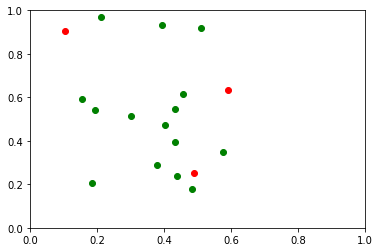
\includegraphics[width=6cm]{Imagens/solucoes-itens.png}
    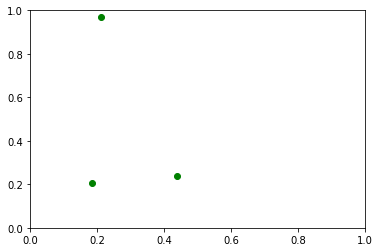
\includegraphics[width=6cm]{Imagens/recommender_item.png}
   \caption{Conjunto de itens e as soluções geradas pelo MOEA (esquerda) e o resultado da recomendação (direita).}
    \label{fig:solucoes_itens}
    
\end{figure}




        